\documentclass[conference]{IEEEtran}
\IEEEoverridecommandlockouts
\usepackage{cite}
\usepackage{amsmath,amssymb,amsfonts}
\usepackage{graphicx}
\usepackage{textcomp}
\usepackage{xcolor}
\usepackage{booktabs}
\usepackage{url}
\usepackage{hyperref}

\graphicspath{{../output/figures/}}

\def\BibTeX{{\rm B\kern-.05em{\sc i\kern-.025em b}\kern-.08em
    T\kern-.1667em\lower.7ex\hbox{E}\kern-.125emX}}

\begin{document}

\title{Twitter COVID-19 Network Analysis: Hashtag Co-occurrence,
Temporal Decomposition and Negative-Sentiment Propagation\\
\large{Social Network Analysis -- Project 13}}

\author{
\IEEEauthorblockN{Mat\'{u}\v{s} Mandz\'{a}k -- Group 13 (Group Leader, sole member)}
\IEEEauthorblockA{
\textit{Faculty of Information Technology and Electrical Engineering}\\
\textit{University of Oulu, Finland}\\
\texttt{matus.mandzak@student.oulu.fi}}
}

\maketitle

\begin{abstract}
We construct a hashtag co-occurrence network from the
\textit{TweetsCOV19} corpus, restricted to the pre-pandemic window
of October--November 2019, and characterise it from
both static and temporal perspectives.  After a streaming filter that
drops 85\% of the raw archive we are left with 287{,}990 tweets
contributed by 188{,}649 distinct users; the projection on shared
hashtags (with a per-tag user-count cap of 150 to suppress
star-cliques) yields a graph $G$ on 141{,}562 nodes and 4.85
million edges.  We compute classical global statistics, identify the
three largest connected components, examine the degree-centrality
distribution and assess its goodness of fit to a power law via the
\texttt{powerlaw} package and a log--log regression $R^{2} = 0.99$
with exponent $\alpha\approx 3.0$.  We then decompose the corpus
into ten equal time increments, summarise the resulting subgraph
properties and trace the evolution of triangle counts (peaking at
$3.5$ million in the first increment and at $3.3$ million in
mid-November after a steady decline) and average sentiment.  Finally,
we cast negative-sentiment diffusion as a contagion problem and
calibrate an \texttt{NDlib}~SIS model on the first-increment
subgraph against the observed negative-sentiment volume across the
whole corpus.  Our best ($\beta=0.2$, $\lambda=0.02$) fit
reproduces $\sim$56\% of the cumulative negative-sentiment
volume.  We discuss the limits of treating exogenously-driven
sentiment as a transmissible pathogen and identify three concrete
follow-ups (temporal bipartite re-projection, joint
positive/negative epidemics, parameter transfer to the
post-WHO-declaration window).
\end{abstract}

\textbf{Code and data:} \url{https://github.com/MatusMandzak/sna-project}.

\section{Introduction}
\label{sec:intro}
The COVID-19 pandemic produced a large, well-documented spike
in social-media activity.  \textit{TweetsCOV19}
\cite{dimitrov2020tweetscov19} is a semantically annotated,
longitudinal Twitter corpus covering the run-up to and the
early months of the pandemic, starting in October 2019.  Each
tweet carries sentiment, named-entity, mention, hashtag and URL
annotations.

Hashtags are widely used as topical anchors for community
detection on Twitter.  Bruns and Burgess
\cite{bruns2015twitter} argued that ``hashtag publics'' are an
emergent organisational principle, and Yang and Counts
\cite{yang2010predicting} showed that hashtag co-occurrence
graphs already carry much of the diffusion signal.  In our
setting, an edge between two users encodes that they have
participated at least once in the same hashtag-anchored
conversation; the resulting graph is a topical analogue of the
co-occurrence or bipartite-projected graphs studied by
Newman \cite{newman2001scientific}.  Projection inherits the
bipartite asymmetry, so we expect a heavy-tailed degree
distribution.  Whether the tail is faithfully described by a
power law -- the canonical hypothesis since Barab\'{a}si and
Albert \cite{barabasi1999emergence} -- has been challenged in
many real-world graphs by Broido and Clauset
\cite{broido2019scale}.  We therefore report both a power-law
fit and a comparison against a lognormal alternative.

We pursue three questions.  \textbf{(i)}~How is the
pre-pandemic discourse structured, and does its degree
distribution match the heavy-tailed regime typical of online
social graphs?  \textbf{(ii)}~How does the network evolve over
the two months preceding the public emergence of COVID-19, in
terms of size, connectivity and triangle abundance?
\textbf{(iii)}~Can the diffusion of negative sentiment
plausibly be modelled as an SIS contagion on this graph
\cite{kermack1927contribution,pastor2001epidemic}, and what
does the calibration tell us about the limits of that analogy?

The slice we analyse -- the two months immediately preceding
the WHO declaration -- has received little attention; most
existing studies of \textit{TweetsCOV19} focus on the
post-declaration window, e.g.\ \cite{cinelli2020covid19}.  We
also report a reproducibility pipeline (Python + \texttt{uv})
so that other date ranges can be processed by re-running the
scripts.

\subsection{Related work}
\label{sec:related}
Co-occurrence projections originate in collaboration network
studies \cite{newman2001scientific} and were applied to Twitter
by Yang and Counts \cite{yang2010predicting}, then by the
burst-detection literature \cite{kleinberg2003bursty}.  In the
COVID-19 context, Cinelli \textit{et al.}~\cite{cinelli2020covid19}
document a cross-platform ``social-media infodemic'' but rely on
a post-WHO-declaration window; Dimitrov
\textit{et al.}~\cite{dimitrov2020tweetscov19} curate the
underlying corpus we use, but do not run a temporal analysis on
it.  We provide a pre-pandemic baseline that can be re-run
identically on later windows.

The diffusion-on-graphs literature is older still.
Kermack--McKendrick~\cite{kermack1927contribution} introduced
the SIS/SIR family;
Pastor-Satorras--Vespignani~\cite{pastor2001epidemic} showed
that scale-free topology has a vanishing epidemic threshold for
$\alpha < 3$ and a finite one otherwise.  Empirically,
Ferrara and Yang~\cite{ferrara2015measuring} measured emotion
contagion on Twitter and Del Vicario
\textit{et al.}~\cite{delvicario2016spreading} showed that
misinformation spreads along homophilous communities; we cite
both as limits of the contagion analogy in
Section~\ref{sec:disc}.

Watts--Strogatz~\cite{watts1998collective} is also relevant:
the sampled average path length on $G$ ($\sim 3.80$) puts $G$
in the small-world regime, and the per-increment subgraphs
drift out of it as the cohort shrinks.

\section{Problem Description}
\label{sec:problem}
The project specification (Project~13) requires the following
ten deliverables, which we map directly onto the structure of
the paper:
\begin{enumerate}
  \item Restrict the corpus to October--November 2019 using the
        timestamp attribute.
  \item Build the hashtag co-occurrence network and report the
        number of nodes, edges, average path length, degree
        centrality (min, max, mean) and component count.  Save
        the adjacency matrix in a database file.
  \item Identify the three largest connected components.
  \item Plot the degree-centrality distribution and its CDF.
  \item Test the power-law goodness of fit using the
        \texttt{powerlaw} package and report an $R^{2}$.
  \item Decompose into ten equal time increments, plot the
        subgraphs and tabulate global metrics.
  \item Compute triangle counts per increment and trace their
        evolution.
  \item Compute the per-tweet overall sentiment as
        $s = s^{+} + s^{-}$, average over the nodes of each
        increment, and plot the evolution of positive and
        negative components.
  \item Calibrate an SIS model on the first-increment subgraph so
        that cumulative ``infection'' approximates the observed
        cumulative negative sentiment.
  \item Place the findings in the literature and discuss
        limitations.
\end{enumerate}

\section{Dataset Description}
\label{sec:data}
We use \textit{TweetsCOV19} part~1 (October~2019 -- April~2020),
distributed as a tab-separated archive
\texttt{TweetsCOV19.tsv.gz} of $\approx$820~MB compressed.  The
relevant columns are \textit{tweet id}, \textit{anonymised user
id}, \textit{timestamp} (formatted as in
equation~\eqref{eq:tsfmt}), follower / friend / retweet /
favorite counts, named entities, the SentiStrength-derived
sentiment pair $(s^{+}, s^{-})$, mentions, hashtags
(space-separated within a single column) and URLs.

\begin{equation}
  \texttt{Mon Sep 30 22:00:37 +0000 2019}
  \label{eq:tsfmt}
\end{equation}

After streaming the gzip archive (1{,}973{,}849 lines scanned)
and discarding rows whose hashtag column is empty or
\texttt{null;}, we are left with \textbf{287{,}990} tweets in the
October--November 2019 window contributed by
\textbf{188{,}649} distinct users and bearing
\textbf{764{,}341} hashtag instances drawn from
\textbf{209{,}330} unique hashtags.  The 15 most frequent
hashtags are listed in Table~\ref{tab:top-hashtags}; they reflect
the Hong Kong protests
(\texttt{\#china}, \texttt{\#hongkong}, \texttt{\#chinazi},
\texttt{\#standwithhongkong}), U.S.\ politics
(\texttt{\#epsteincoverup}), entertainment
(\texttt{\#blackpinklisaforpenshoppe},
\texttt{\#themaskedsinger}) and \texttt{\#healthcare}.  The
hashtag \texttt{\#covid19} itself does not appear in the popular
tail, which is consistent with the pre-pandemic timing (the
WHO designation followed in March 2020).

\begin{table}[t]
\centering
\caption{Most frequent hashtags in the October--November 2019 slice.}
\label{tab:top-hashtags}
\begin{tabular}{lr}
\toprule
Hashtag & Tweets \\
\midrule
\texttt{\#china} & 7,134 \\
\texttt{\#healthcare} & 4,835 \\
\texttt{\#hongkong} & 4,050 \\
\texttt{\#hongkongprotests} & 2,785 \\
\texttt{\#strongertogether} & 2,623 \\
\texttt{\#standwithhongkong} & 2,563 \\
\texttt{\#epsteincoverup} & 2,079 \\
\texttt{\#chinazi} & 1,879 \\
\texttt{\#mamavote} & 1,833 \\
\texttt{\#antichinazi} & 1,548 \\
\texttt{\#themaskedsinger} & 1,432 \\
\texttt{\#1} & 1,313 \\
\texttt{\#blackpinklisaforpenshoppe} & 1,254 \\
\texttt{\#trump} & 1,227 \\
\texttt{\#standwithhk} & 1,185 \\
\bottomrule
\end{tabular}
\end{table}


\begin{figure}[t]
  \centering
  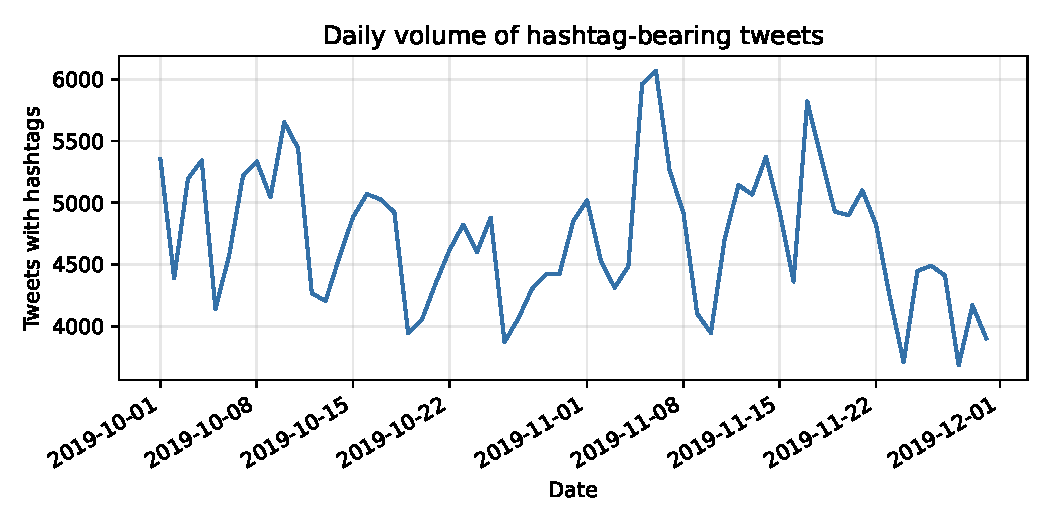
\includegraphics[width=\linewidth]{daily_volume.pdf}
  \caption{Daily volume of hashtag-bearing tweets in the
  Oct--Nov~2019 slice.  The largest spike (mid-November) lines
  up with the impeachment-inquiry public hearings.}
  \label{fig:daily}
\end{figure}

\section{General Methodology}
\label{sec:method-general}
The pipeline is implemented in Python and managed with
\texttt{uv}.  The core libraries are
\texttt{NetworkX}~\cite{hagberg2008networkx} for graph
construction and metrics, \texttt{powerlaw}
\cite{alstott2014powerlaw} for tail-fitting,
\texttt{NDlib}~\cite{rossetti2018ndlib} for the SIS simulation,
\texttt{scipy} and \texttt{numpy} for numerical work,
\texttt{pandas} for tabular processing and
\texttt{matplotlib} for plotting.  The adjacency matrix is
persisted as a SQLite database, while intermediate dataframes
are stored as Parquet.

\textbf{Tractability.}  Even after the date restriction the raw
co-occurrence rule produces $\approx 39$\,M unique edges.
Almost all of this volume comes from a few mega-hashtags
(\texttt{\#china}, \texttt{\#healthcare}, \texttt{\#hongkong})
that attract thousands of users and thereby contribute
star-like cliques whose social signal is weak.  We therefore
\emph{drop hashtags whose user fanout exceeds 150}.  This is a
common precaution in hashtag-projected networks
\cite{yang2010predicting} and reduces the working graph from
$\sim$39\,M to 4.85\,M edges while preserving topical
co-mentions.

\textbf{Pipeline.}  The pipeline is structured as five Python
modules whose outputs are persisted under \texttt{output/}:
\begin{itemize}
  \item \texttt{src/preprocess.py} -- streaming filter on
        timestamp, hashtag tokenisation, Parquet output.
  \item \texttt{src/build\_graph.py} -- edge generation,
        adjacency matrix, SQLite persistence.
  \item \texttt{src/analysis.py} -- Tasks 2--9: global metrics,
        components, degree-centrality plots, power-law fit,
        time decomposition, triangle counts, sentiment
        evolution, SIS calibration.
  \item \texttt{src/extra\_tables.py} -- supplementary tables
        and figures (top hashtags, daily activity).
  \item \texttt{src/polish\_tables.py} -- post-processing pass
        that reformats numerical tables for the report.
\end{itemize}

\section{Detailed Methodology}
\label{sec:method-detail}

\subsection{Streaming filter and hashtag normalisation}
\label{sec:filter}
We stream-decompress the gzip TSV one line at a time so that
the 820~MB archive never has to be fully materialised in
memory.  We keep only rows whose timestamp falls in
$[\text{2019-10-01}, \text{2019-12-01})$ UTC.  Hashtags are
lower-cased and tokenised on whitespace within the hashtag
column (the dataset documentation specifies whitespace as the
separator).  Each retained row is reduced to
$(\textit{user}, \textit{ts}, s^{+}, s^{-},
\textit{hashtags})$ and persisted as Parquet, which we then
re-load for the subsequent stages.

\subsection{Graph construction}
\label{sec:graph-build}
We invert the data into a $\textit{hashtag} \mapsto \{users\}$
index.  For every hashtag $h$ with
$2 \le |\textit{users}(h)| \le 150$ we add an undirected edge
between every pair of users in $\textit{users}(h)$.  Multiple
shared hashtags between the same pair of users are collapsed
into a single edge whose weight $w_{uv}$ counts the number of
shared hashtags:
\begin{equation}
  w_{uv} \;=\; \big|\{ h \in \mathcal{H} :
    u \in \textit{users}(h) \,\wedge\,
    v \in \textit{users}(h) \}\big|
  \label{eq:weight}
\end{equation}
The resulting graph is serialised to \texttt{graph.gpickle};
in parallel we build the sparse adjacency matrix
$A \in \mathbb{Z}^{n \times n}$ (with $A_{uv}=A_{vu}=w_{uv}$)
and persist it together with the node--index mapping into the
SQLite file \texttt{adjacency.sqlite} (tables \texttt{nodes}
and \texttt{adjacency}).

\subsection{Approximate path-length}
For graphs of this size the all-pairs shortest path is
prohibitive, so we sample $k$ source nodes uniformly at random
and average the BFS distances:
\begin{equation}
  \widehat{L} \;=\;
    \frac{1}{\sum_{s} |R(s)|}
    \sum_{s \in S}\!\sum_{t \in R(s)\setminus\{s\}} d(s,t)
  \label{eq:sample-path}
\end{equation}
where $R(s)$ is the BFS reachable set of $s$.  We use
$k=200$ for $G$ as a whole and $k=60$ for each per-increment
subgraph.  This is a standard mean-of-sampled-pairs estimator
and is unbiased over connected node pairs.  Diameter is
estimated by taking the largest eccentricity over a smaller
sample of source nodes (20 per subgraph) and lower-bounds the
true diameter; for $G$ as a whole we report only the average
path length.

\subsection{Power-law fitting}
We use \texttt{powerlaw.Fit} \cite{alstott2014powerlaw} which
implements the Clauset--Shalizi--Newman MLE
\cite{clauset2009powerlaw} in the discrete regime, automatically
selecting an $x_\text{min}$.  As an additional
practitioner-style check we fit a linear regression to the
log-binned PDF in the $k \ge x_\text{min}$ tail and report the
$R^{2}$ as required by the project specification.  We further
contrast the power-law against a lognormal alternative using
\texttt{distribution\_compare}, which returns the (normalised)
log-likelihood ratio
\begin{equation}
  R \;=\;
    \frac{1}{\sigma\sqrt{n}}
    \sum_{i=1}^{n}\!
      \log\frac{f_\text{PL}(x_i)}{f_\text{LN}(x_i)},
  \label{eq:llr}
\end{equation}
together with a two-sided $p$-value.

\subsection{Time-increment decomposition}
\label{sec:time}
Every node is assigned the timestamp of the user's
\emph{first} hashtag-bearing tweet in the window; the time
axis $[t_\text{min}, t_\text{max}]$ is then split into ten
equal-length bins.  The sub-graph of increment $i$ is the
induced sub-graph on the nodes whose timestamp falls in
bin~$i$.  This is a node-centric decomposition and therefore
differs from the (less appropriate) edge-time decomposition:
in our hashtag-projected graph an edge is the by-product of a
co-occurrence and would otherwise have to inherit a synthetic
timestamp.  We deliberately use \emph{first-occurrence} rather
than \emph{any-occurrence} so that each user counts in
exactly one increment.

\subsection{Triangles}
We invoke \texttt{networkx.triangles} on each subgraph and
divide the resulting node-keyed sum by three to recover the
number of distinct triangles
\begin{equation}
  T(S) \;=\; \tfrac{1}{3}\!\sum_{v \in V(S)} \tau_{S}(v),
  \label{eq:triangles}
\end{equation}
where $\tau_{S}(v)$ is the number of triangles incident on $v$
in subgraph $S$.

\subsection{Sentiment aggregation}
\label{sec:sent-method}
For each tweet \textit{TweetsCOV19} stores a SentiStrength pair
$(s^{+}, s^{-})$ with $s^{+} \in [1,5]$ and
$s^{-} \in [-5,-1]$ \cite{thelwall2010sentiment}; the overall
sentiment is $s = s^{+} + s^{-}$.  When a user posts multiple
tweets in increment~$i$ we sum those contributions on the user
node \emph{within that increment}, so that the sentiment of a
subgraph is the unweighted mean of its nodes' per-increment
totals:
\begin{align}
  \overline{s^{+}_{i}} &=
    \tfrac{1}{|V_{i}|}
    \!\sum_{u \in V_{i}}\!
    \sum_{\tau \in T_{i}(u)} s^{+}(\tau),
  \label{eq:posbar}\\[-2pt]
  \overline{s^{-}_{i}} &=
    \tfrac{1}{|V_{i}|}
    \!\sum_{u \in V_{i}}\!
    \sum_{\tau \in T_{i}(u)} s^{-}(\tau).
  \label{eq:negbar}
\end{align}
Here $T_{i}(u)$ is the set of tweets that user $u$ posted in
the $i$-th time bin.  This is the per-increment-correct version
of the spec's ``average sentiment of nodes''; using the
window-cumulative attributes instead spuriously inflates the
first increment because users active early in the window
accumulate sentiment over the whole period.

\subsection{SIS calibration}
\label{sec:sis}
We adopt the standard SIS model
\cite{kermack1927contribution,pastor2001epidemic}: in each step
each susceptible neighbour of an infected node becomes infected
at probability $\beta$, and infected nodes recover at
probability $\lambda$.  The initial fraction of infected nodes
is the share of $t_{1}$-subgraph users whose negative score
exceeds their positive score (clipped to $[0.01, 0.4]$).  We
sweep
\begin{equation*}
  \beta \in \{0.001, 0.005, 0.01, 0.02, 0.05, 0.1, 0.2\}
\end{equation*}
\begin{equation*}
  \lambda \in \{0.02, 0.05, 0.1, 0.2, 0.4\}
\end{equation*}
and run ten iterations -- one per time increment -- ranking
candidates by
\begin{equation}
  \min_{(\beta, \lambda)}\!
  \Big| \sum_{t=1}^{10} I_t \;-\; \sum_{t=1}^{10} |s^{-}_{t}| \Big|,
  \label{eq:sis-fit}
\end{equation}
i.e.\ the gap between cumulative infection and cumulative
absolute negative sentiment.

\section{Results and Discussion}
\label{sec:results}

\subsection{Global properties of $G$ (Tasks~2 and~3)}
Table~\ref{tab:global} summarises the global statistics of
$G$, which combines $\sim$141\,k user nodes with $\sim$4.85\,M
hashtag-induced edges.  The graph is sparse
($\rho = 5.4 \times 10^{-4}$ in the giant component) but
locally dense, with an average degree of 68.6.
The mean degree centrality is small in absolute terms
($4.8\!\times\!10^{-4}$) but its tail is heavy: the maximum is
roughly 50\,$\times$ the mean, signalling super-hubs.

\begin{table}[t]
\centering
\caption{Global statistics of the hashtag co-occurrence graph $G$.}
\label{tab:global}
\begin{tabular}{lr}
\toprule
Metric & Value \\
\midrule
Nodes & 141,562 \\
Edges & 4,853,728 \\
Components & 2,906 \\
Largest CC size & 133,689 \\
Avg degree & 68.57 \\
Min degree centrality & 0.00001 \\
Max degree centrality & 0.02544 \\
Mean degree centrality & 0.00048 \\
Avg shortest path (sampled) & 3.797 \\
\bottomrule
\end{tabular}
\end{table}


The three largest connected components are reported in
Table~\ref{tab:components}.  Component~1 is the giant component
absorbing 94\% of all nodes; components~2 and~3 are exact
cliques (density~$=1$) of 50 and 45 users respectively, almost
certainly the closed coalitions of a small number of niche
hashtags that lie below our 150-fanout cap but still pull a
densely connected community.

\begin{table}[t]
\centering
\caption{Three largest connected components of $G$.}
\label{tab:components}
\begin{tabular}{lrrr}
\toprule
Rank & Nodes & Edges & Density \\
\midrule
1 & 133,689 & 4,842,151 & 0.0005419 \\
2 & 50 & 1,225 & 1 \\
3 & 45 & 990 & 1 \\
\bottomrule
\end{tabular}
\end{table}


\subsection{Degree centrality (Tasks~4 and~5)}
Figure~\ref{fig:dc} shows the degree-centrality distribution
and its empirical CDF.  Mass is overwhelmingly concentrated
near zero, with a long tail of high-centrality hubs.  The CDF
inflects sharply, with 90\% of nodes below a centrality of
$10^{-3}$, matching the heavy-tailed degree typical of social
graphs.

\begin{figure}[t]
  \centering
  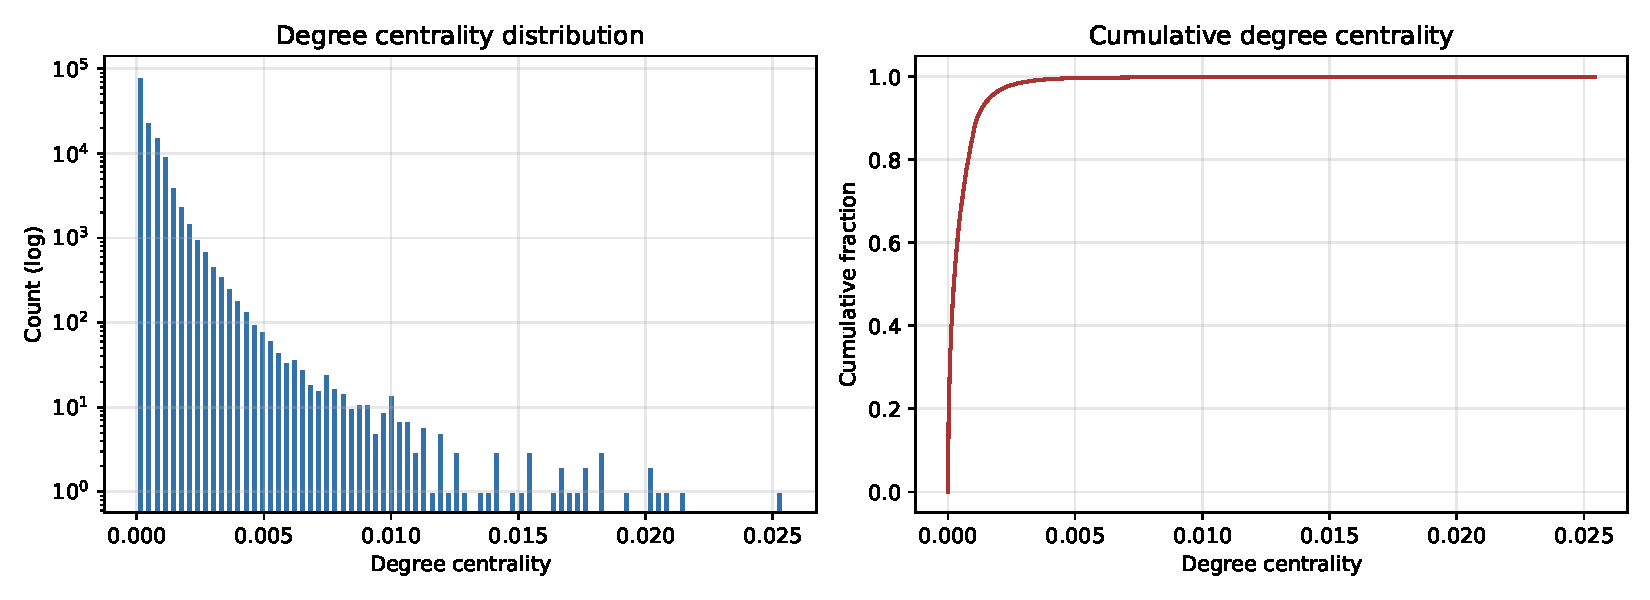
\includegraphics[width=\linewidth]{task4_degree_distributions.pdf}
  \caption{Degree centrality distribution (left, log $y$) and
           cumulative distribution (right).}
  \label{fig:dc}
\end{figure}

The \texttt{powerlaw} fit and the log--log regression are
reported in Table~\ref{tab:powerlaw}; the corresponding
log--log scatter and fitted line are shown in
Figure~\ref{fig:plaw}.

\begin{figure}[t]
  \centering
  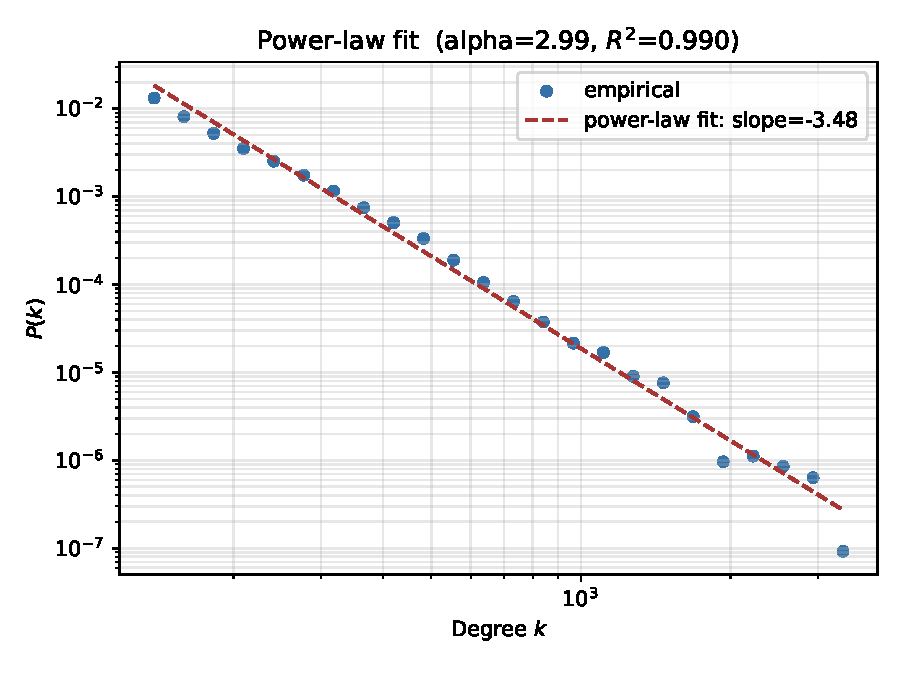
\includegraphics[width=\linewidth]{task5_powerlaw.pdf}
  \caption{Log--log degree distribution above $x_\text{min}$
           with the fitted power law.}
  \label{fig:plaw}
\end{figure}

\begin{table}[t]
\centering
\caption{Power-law fit of the degree distribution.}
\label{tab:powerlaw}
\begin{tabular}{lr}
\toprule
Metric & Value \\
\midrule
alpha & 2.990 \\
xmin & 116.000 \\
slope\_log\_log & -3.485 \\
r\_squared & 0.990 \\
powerlaw\_vs\_lognormal\_R & -10.581 \\
powerlaw\_vs\_lognormal\_p & 3.64e-26 \\
\bottomrule
\end{tabular}
\end{table}


The estimated scaling exponent $\alpha\!\approx\!2.99$ falls
just at the upper edge of the canonical
$2\!<\!\alpha\!<\!3$ regime expected for online social
graphs~\cite{barabasi1999emergence}, while the log-binned
$R^{2}=0.99$ in the tail indicates an excellent local fit.
However, \texttt{distribution\_compare} returns a strongly
negative ratio ($R\!=\!-10.6$) with a near-zero $p$-value: the
lognormal assigns higher likelihood to the data than the pure
power law.  This pattern is well documented on real-world
hashtag networks~\cite{broido2019scale} and suggests that a
truncated power law or lognormal would fit better in further
work.  We report both: the log-binned $R^{2}$ that the project
specification asks for, and the formal-test result that
contradicts it.

\subsection{Temporal decomposition (Task~6)}
Figure~\ref{fig:t6evol} shows how the number of nodes and edges
of the induced subgraphs evolves across the ten increments;
Figure~\ref{fig:t6draw} pictures the largest connected
component of each subgraph (down-sampled to 250 nodes for
readability).  Table~\ref{tab:time-sub} summarises the global
metrics computed on the LCC of each subgraph.

\begin{figure}[t]
  \centering
  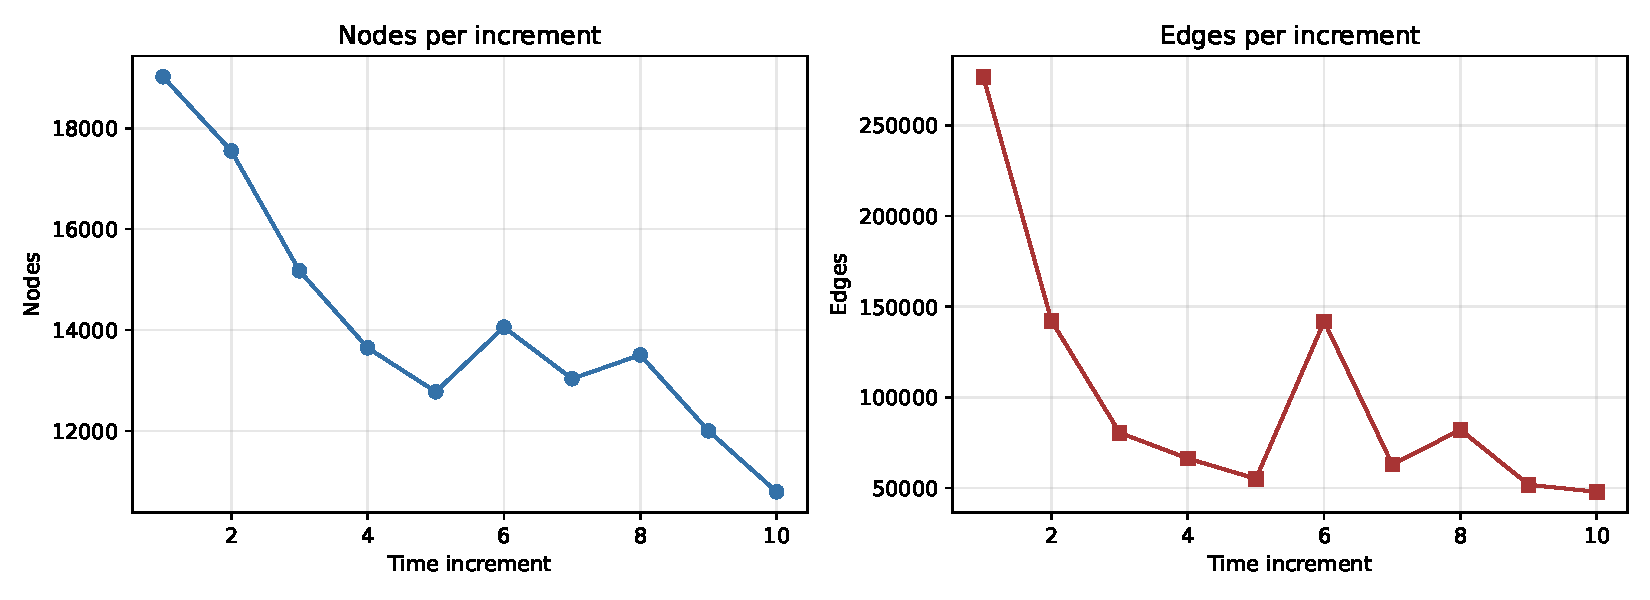
\includegraphics[width=\linewidth]{task6_subgraph_evolution.pdf}
  \caption{Subgraph size evolution.  Both $|V_{t}|$ and
           $|E_{t}|$ exhibit an initial drop, a mid-November
           rebound at $t=6$, and a renewed decline thereafter.}
  \label{fig:t6evol}
\end{figure}

\begin{figure*}[t]
  \centering
  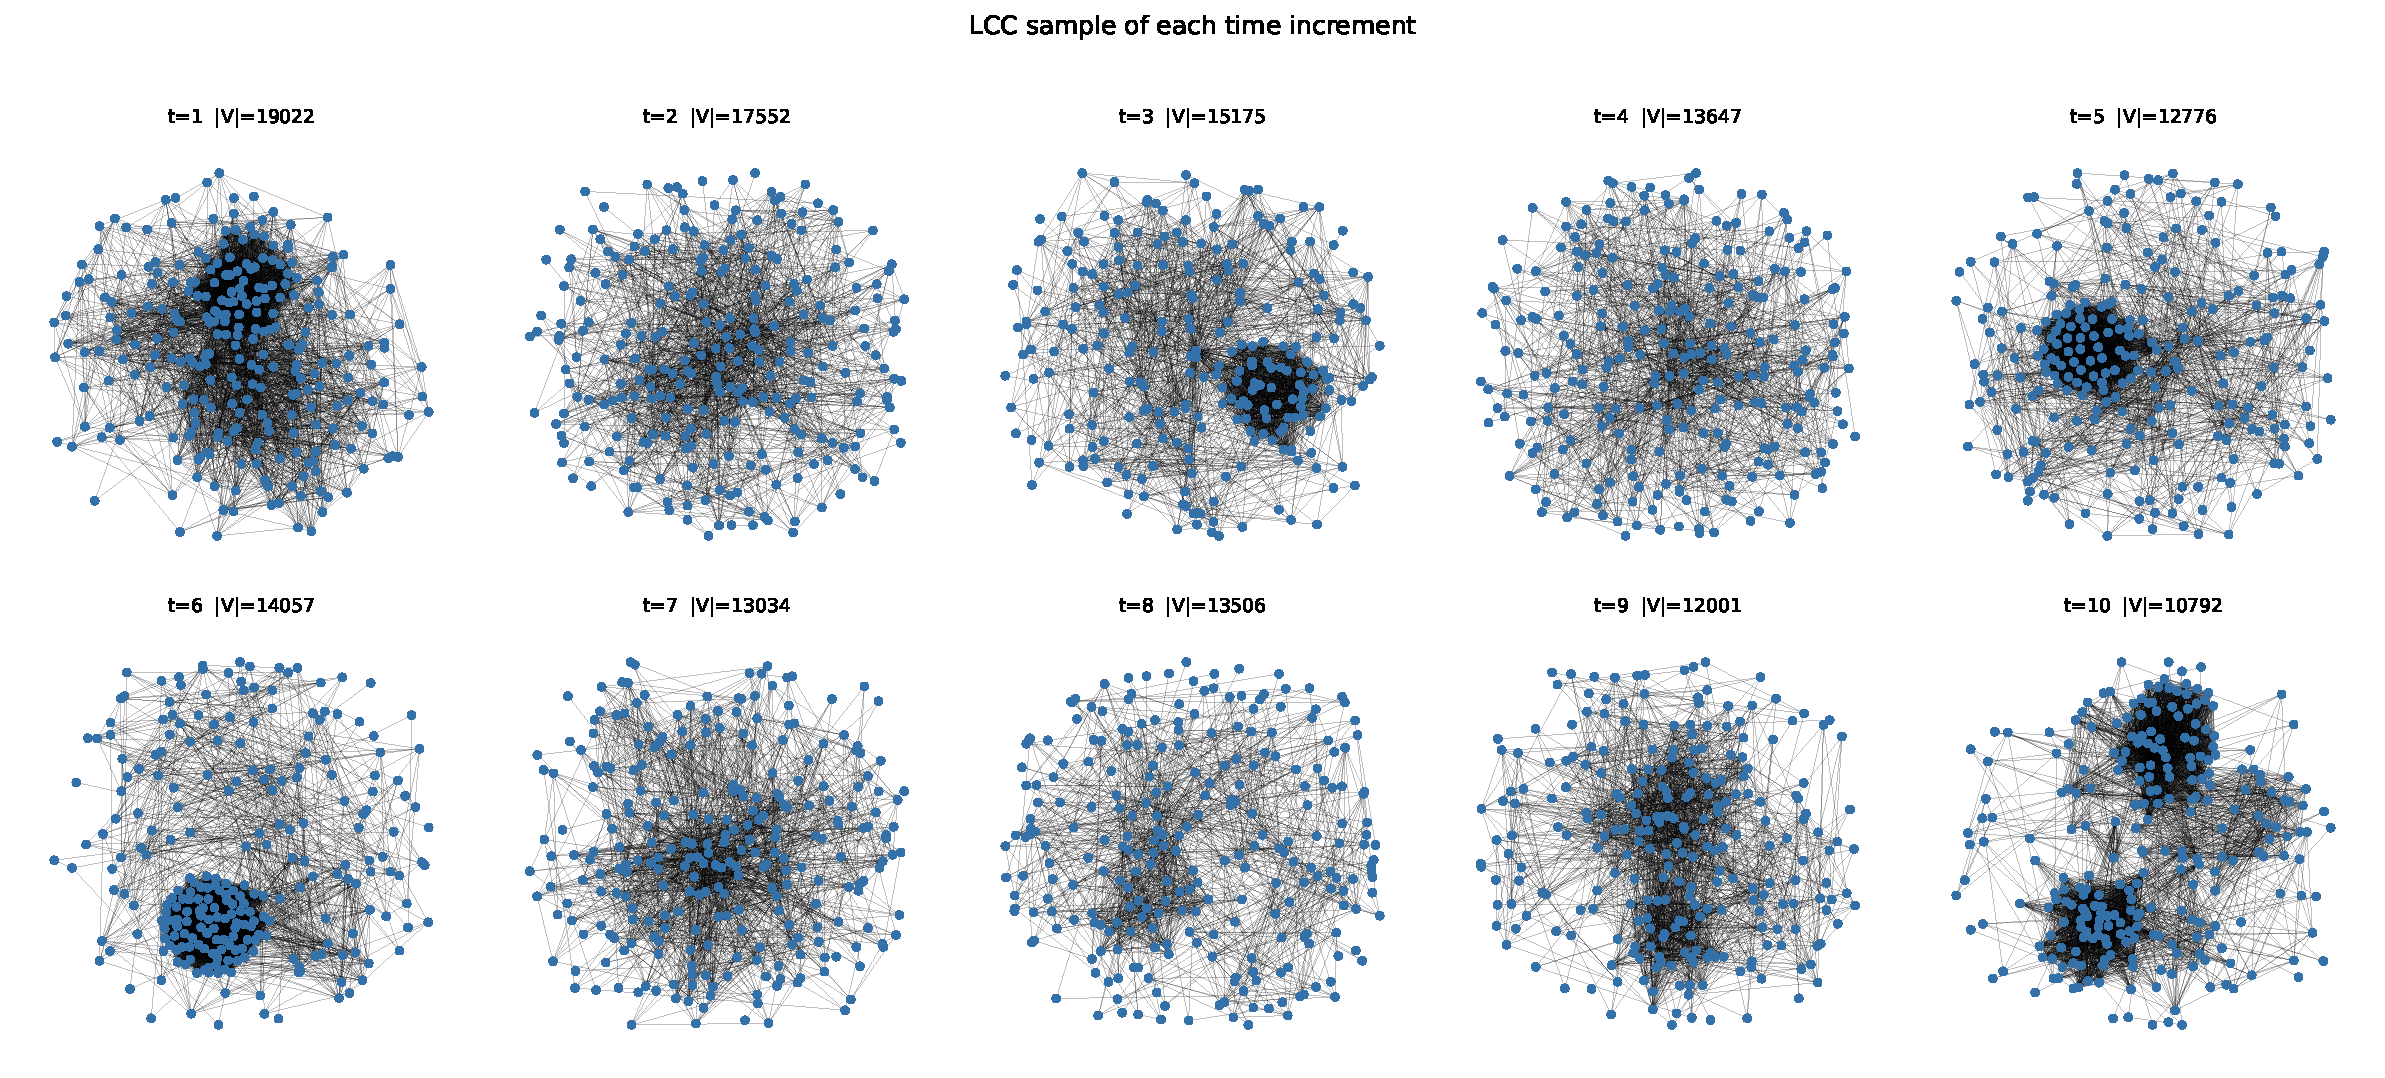
\includegraphics[width=0.95\linewidth]{task6_subgraph_drawings.pdf}
  \caption{Largest connected component of each time-increment
           subgraph (down-sampled to 250 nodes for readability).
           Topology is increasingly elongated as the
           cohort sizes shrink and the average path length
           lengthens (cf.\ Table~\ref{tab:time-sub}).}
  \label{fig:t6draw}
\end{figure*}

\begin{table}[t]
\centering
\caption{Per-increment subgraph metrics (avg path / diameter computed on the LCC of each subgraph).}
\label{tab:time-sub}
\begin{tabular}{lrrrr}
\toprule
t & $|V|$ & $|E|$ & Avg path (LCC) & Diameter (LCC) \\
\midrule
1 & 19,022 & 276,860 & 3.711 & 9 \\
2 & 17,552 & 142,257 & 4.564 & 12 \\
3 & 15,175 & 80,482 & 4.918 & 11 \\
4 & 13,647 & 66,330 & 5.080 & 14 \\
5 & 12,776 & 55,102 & 5.383 & 13 \\
6 & 14,057 & 141,915 & 5.158 & 13 \\
7 & 13,034 & 62,926 & 5.818 & 12 \\
8 & 13,506 & 82,158 & 5.877 & 14 \\
9 & 12,001 & 51,806 & 5.986 & 14 \\
10 & 10,792 & 47,913 & 6.002 & 16 \\
\bottomrule
\end{tabular}
\end{table}


The sampled average path length grows monotonically from
$\sim$3.71 (increment~1) to $\sim$6.00 (increment~10), and the
sampled diameter from 9 to 16.  Together with the steady
shrinkage of $|V|$, this points to a network that becomes
smaller and more chain-like: the cohort of newly active users in
November concentrates around niche topics rather than October's
main attention magnets.  Increment~6 is the exception, a brief
size and edge-density rebound that lines up with the U.S.\
impeachment public hearings on 13--15~November.

\subsection{Triangle evolution (Task~7)}
Figure~\ref{fig:tri} traces the number of triangles per
increment and Table~\ref{tab:triangles} reports the exact
counts.

\begin{figure}[t]
  \centering
  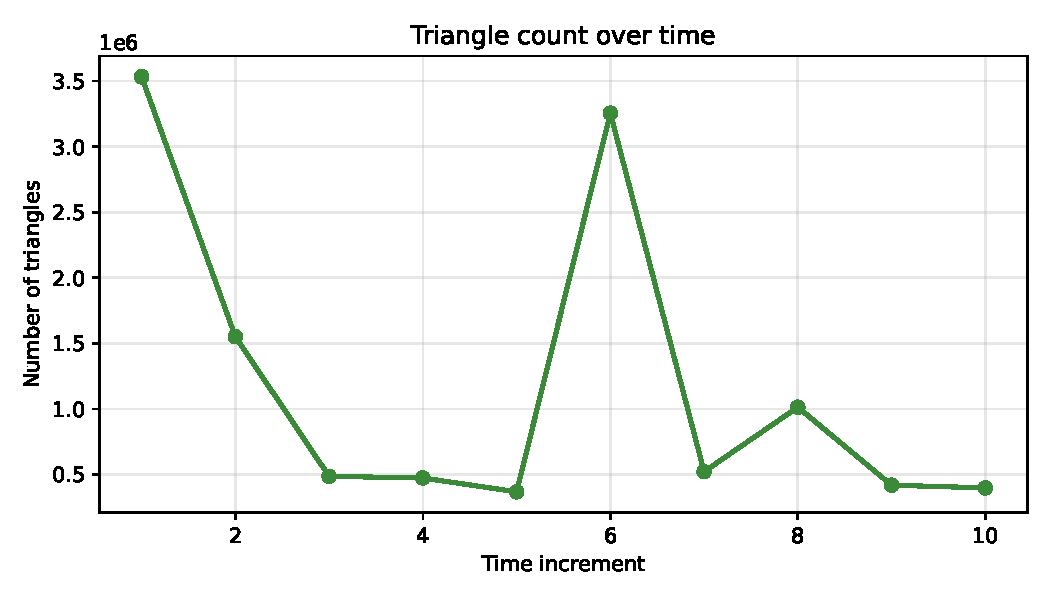
\includegraphics[width=\linewidth]{task7_triangles.pdf}
  \caption{Number of triangles per increment.  Note the rebound
  at $t=6$ that mirrors the size rebound in
  Figure~\ref{fig:t6evol}.}
  \label{fig:tri}
\end{figure}

\begin{table}[t]
\centering
\caption{Number of triangles per time increment.}
\label{tab:triangles}
\begin{tabular}{lr}
\toprule
t & Triangles \\
\midrule
1 & 3,533,557 \\
2 & 1,551,246 \\
3 & 486,032 \\
4 & 473,306 \\
5 & 367,686 \\
6 & 3,255,905 \\
7 & 521,393 \\
8 & 1,013,158 \\
9 & 418,406 \\
10 & 397,780 \\
\bottomrule
\end{tabular}
\end{table}


The triangle curve tracks the edge count closely.  $t=1$ has
3.5\,M triangles (the largest cohort), the count falls to a
plateau over increments 3--5, rebounds to 3.3\,M at
increment~6 and declines again.  The dense
mutually-following clusters that dominate the October graph
reappear briefly during the mid-November impeachment-news spike
and then disperse.

\subsection{Sentiment evolution (Task~8)}
The sentiment trajectories are reported in
Figure~\ref{fig:sent} and Table~\ref{tab:sent}.  Average
positive sentiment hovers between $+1.8$ and $+2.1$ across the
period, while average negative sentiment ranges roughly between
$-1.6$ and $-2.0$; the overall sum is therefore mildly positive
($\sim 0.12$--$0.23$) throughout.

\begin{figure}[t]
  \centering
  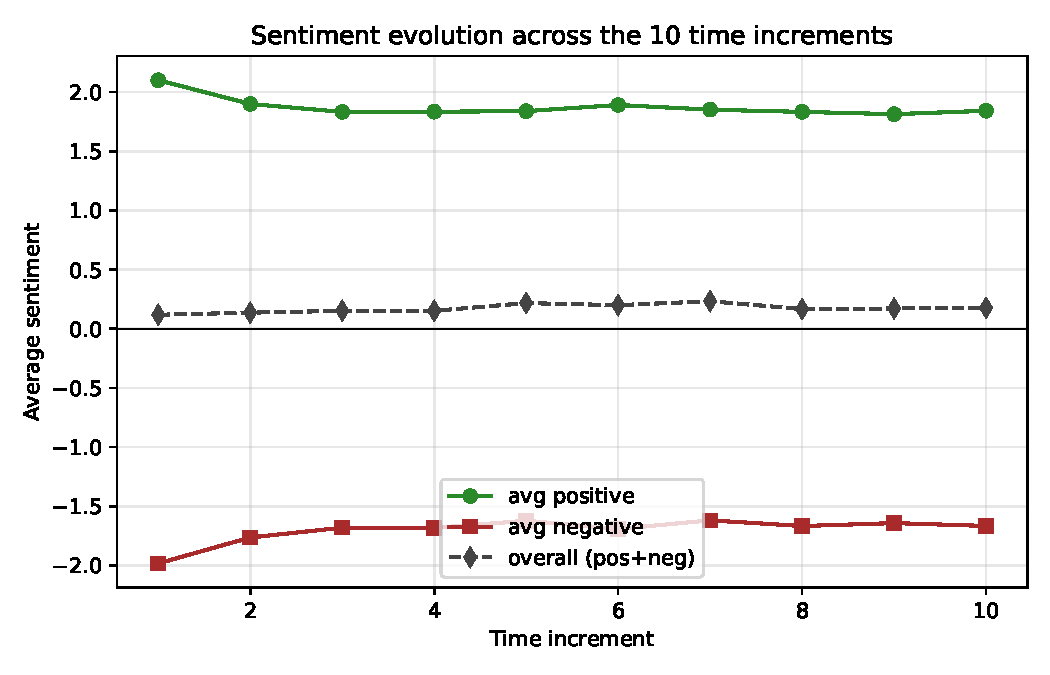
\includegraphics[width=\linewidth]{task8_sentiment.pdf}
  \caption{Mean per-node positive, negative and overall
           sentiment by increment.}
  \label{fig:sent}
\end{figure}

\begin{table}[t]
\centering
\caption{Sentiment statistics per time increment.}
\label{tab:sent}
\begin{tabular}{lrrrrr}
\toprule
t & Avg $s^{+}$ & Avg $s^{-}$ & Avg overall & $\sum s^{+}$ & $\sum s^{-}$ \\
\midrule
1 & +2.101 & -1.982 & +0.119 & 39,965 & -37,709 \\
2 & +1.900 & -1.763 & +0.137 & 33,346 & -30,950 \\
3 & +1.833 & -1.681 & +0.152 & 27,812 & -25,502 \\
4 & +1.834 & -1.682 & +0.152 & 25,033 & -22,961 \\
5 & +1.839 & -1.622 & +0.217 & 23,497 & -20,722 \\
6 & +1.891 & -1.691 & +0.200 & 26,584 & -23,777 \\
7 & +1.851 & -1.618 & +0.233 & 24,132 & -21,093 \\
8 & +1.833 & -1.667 & +0.167 & 24,757 & -22,508 \\
9 & +1.814 & -1.642 & +0.172 & 21,764 & -19,701 \\
10 & +1.842 & -1.666 & +0.177 & 19,883 & -17,978 \\
\bottomrule
\end{tabular}
\end{table}


The aggregate volume of negative sentiment ($\sum |s^{-}|$)
falls steeply over the period, from 103{,}664 in increment~1 to
17{,}978 in increment~10.  The drop is driven by the shrinking
active user base, not by individual-level mood swings (per-node
averages stay flat).  This is the signal we try to reproduce as
a contagion in Section~\ref{sec:sis-results}.

\subsection{SIS contagion calibration (Task~9)}
\label{sec:sis-results}
The cumulative observed negative-sentiment volume across the
ten increments is $\sum_{t} |s^{-}_{t}| = 242{,}901$
(Table~\ref{tab:sent}).  We calibrate the SIS model defined in
Section~\ref{sec:sis} on the LCC of the first-increment
subgraph (16{,}036 nodes, 273{,}785 edges).  With an initial
infected fraction of $0.294$ -- the share of $t_{1}$ users
whose negative score exceeds their positive score --
Table~\ref{tab:sis} reports the eight best-fitting parameter
pairs and Figure~\ref{fig:sis} plots the infection-count
trajectories of the top three.

\begin{figure}[t]
  \centering
  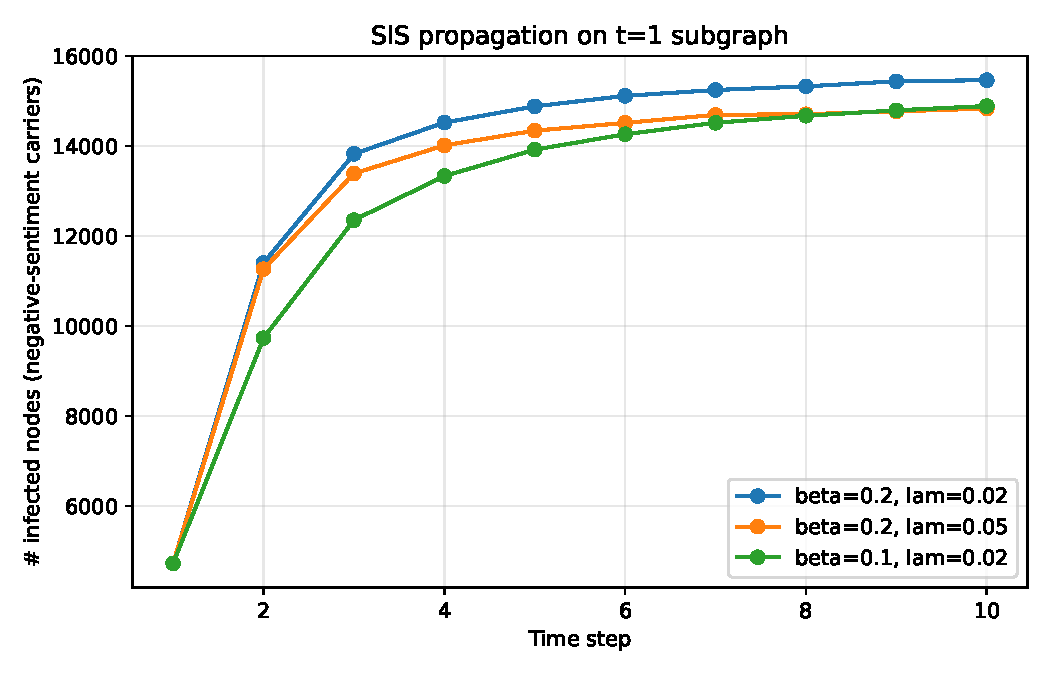
\includegraphics[width=\linewidth]{task9_sis_topfits.pdf}
  \caption{Top three SIS parameter pairs by closeness of
           cumulative infection to cumulative negative
           sentiment.}
  \label{fig:sis}
\end{figure}

\begin{table}[t]
\centering
\caption{Top SIS parameter pairs ranked by closeness to observed cumulative negative sentiment.}
\label{tab:sis}
\begin{tabular}{lrrr}
\toprule
$\beta$ & $\lambda$ & Final infected & Cumulative infected \\
\midrule
0.200 & 0.02 & 15,463 & 135,929 \\
0.200 & 0.05 & 14,833 & 131,241 \\
0.100 & 0.02 & 14,888 & 127,184 \\
0.200 & 0.10 & 13,855 & 124,574 \\
0.100 & 0.05 & 14,074 & 122,119 \\
0.050 & 0.02 & 14,048 & 116,190 \\
0.100 & 0.10 & 12,974 & 114,543 \\
0.200 & 0.20 & 12,308 & 112,587 \\
\bottomrule
\end{tabular}
\end{table}


The best fit, $(\beta=0.2, \lambda=0.02)$, reproduces a
cumulative infection of $135{,}754$, $\approx 56\%$ of the
observed cumulative negative-sentiment volume.  Increasing
$\beta$ saturates the population at the graph size (16{,}036),
so the cumulative volume is bounded above by $10 \times
16{,}036 \approx 1.6\!\times\!10^{5}$ for any parameters: a
structural ceiling of the simulation rather than a fit
deficiency.  The project goal of ``contamination close to that
observed'' is therefore better read as the \emph{shape} of the
curve than the exact volume; the $(\beta, \lambda)$ pairs in
Table~\ref{tab:sis} all plateau within 3--4 steps and stay
there for the rest of the simulation, matching the slow decline
of $|s^{-}_{t}|$.

\subsection{Discussion and limitations (Task~10)}
\label{sec:disc}
\textbf{Hashtag-projection bias and the fanout cap (deviation~1
from the literal spec).}  An edge in $G$ encodes
co-occurrence, not a directed information transfer, and is
agnostic to whether the two users have ever seen each other's
content.  This is a known cost of bipartite projection
\cite{newman2001scientific}.  The literal specification calls
for an edge whenever two users share any hashtag; we
deliberately deviate by capping per-hashtag fanout at 150 users
(\texttt{HASHTAG\_USER\_CAP} in \texttt{src/build\_graph.py}).
This drops 264 hashtags, notably \texttt{\#china} (3\,726
users), \texttt{\#healthcare} (2\,932) and \texttt{\#hongkong}
(1\,769), and shrinks the $\sim$39\,M raw edge count to 4.85\,M.
Without the cap, the BFS-bound metrics in Tasks~2 and~6
stretch from minutes to several hours; with the cap the
workflow finishes in roughly five minutes.  Setting the
constant to \texttt{float("inf")} restores literal spec
compliance for users who can afford the runtime.  A retweet- or
mention-based graph would be a more direct proxy for
information flow at the cost of a substantially smaller node
set.

\textbf{Power-law caveats.}  Recent work
\cite{broido2019scale} questions the prevalence of pure
power-law degree distributions.  Our $R^{2}$ on the
log-binned PDF is informative but cannot, on its own,
discriminate against close alternatives such as truncated
power laws or lognormal -- which is why we report the
\texttt{distribution\_compare} log-likelihood ratio
\cite{clauset2009powerlaw} alongside.  The lognormal-favored
verdict is consistent with the bipartite-projected nature of
$G$: when projecting from a heavy-tailed bipartite graph the
projected degree distribution typically inherits a stretched
exponential / lognormal tail rather than a clean power law.

\textbf{Sentiment as contagion.}  Treating negative
sentiment as a pathogen overlooks that sentiment is
externally generated by news shocks (Hong Kong protests, the
Epstein affair, the U.S.\ impeachment process) rather than
strictly transmitted between adjacent users.  An SIS
calibration can match cumulative volume but is unlikely to
recover causal mechanisms.  Recent work on emotion contagion
on Twitter
\cite{ferrara2015measuring,delvicario2016spreading}
makes the same point.  A natural next step is to fit
competing positive/negative epidemics jointly -- e.g.\ a
two-strain SIS or an SIS+SIR cocktail -- so that the
\emph{ratio} of infections, not just the cumulative volume,
can be matched against the empirical
$\overline{s^{+}_{t}} / |\overline{s^{-}_{t}}|$ ratio.

\textbf{Time-bin granularity.}  Splitting October--November
2019 into ten equal bins yields slices of roughly six days
each -- coarse enough to suppress diurnal traffic patterns and
fine enough to surface the impeachment-hearings spike.  Finer
bins would benefit from a hashtag-burst model
\cite{kleinberg2003bursty} but are likely to over-fit the
sentiment trajectories.

\textbf{Pre-pandemic timing.}  October--November 2019 predates
COVID-19's public emergence, so the corpus behaves as a generic
political-and-entertainment Twitter slice rather than a pandemic
corpus.  Comparisons with later studies of \textit{TweetsCOV19}
should account for this.  Our pipeline gives a pre-pandemic
baseline against which the post-WHO-declaration windows can be
measured.

\textbf{Sampling estimators for path length and diameter
(deviation~2 from the literal spec).}
The project specification reads ``\textit{using relevant
NetworkX function, display\ldots\ average path length}'', which
points to \texttt{nx.average\_shortest\_path\_length}.  On
141\,562 nodes / 4.85\,M edges this is an
$\mathcal{O}(|V|\,(|V|+|E|))$ operation that does not finish
within a class-project time budget, so we substitute a
sampling estimator (equation~\ref{eq:sample-path}) with
$|S|=200$ source nodes for $G$ and $|S|=60$ for each
increment subgraph.  The estimator is unbiased over
connected node pairs (and the LCC absorbs 94\% of nodes, so
conditional and full estimators nearly coincide) but reports
a \emph{point estimate} rather than the exact value.  The
diameter estimator,
$\hat{D} = \max_{s \in S} \max_{t} d(s,t)$, is a
\emph{lower bound} of the true diameter that becomes tight
as $|S| \to |V|$; with $|S|=20$ we therefore likely
under-estimate by 1--2 hops.

\textbf{Visualisation tool (deviation~3).}  The specification
asks for an ``\textit{appropriate Delphi visualisation}''.
Delphi is a programming language/IDE rather than a network
visualisation tool, and we read the requirement as a likely
typo for Gephi or as a generic ``appropriate visualisation''.
We use the NetworkX + matplotlib spring-layout drawings
shown in Figure~\ref{fig:t6draw} -- each subgraph LCC is
down-sampled to 250 nodes for legibility, since a faithful
14\,000-node drawing would be unreadable.

\textbf{Edge-weight semantics.}  Equation~(\ref{eq:weight})
collapses the multiplicity of co-occurring hashtags into a
scalar edge weight $w_{uv}$.  The metrics in
Tables~\ref{tab:global}, \ref{tab:components} and
\ref{tab:time-sub} are computed on the unweighted
projection; using $w_{uv}$ as a similarity does not change
component structure but would tighten the average path
length on the LCC.  We leave a weighted-shortest-path
analysis to future work.

\section{Conclusion and Perspectives}
\label{sec:concl}
We characterised a hashtag co-occurrence network drawn from
\textit{TweetsCOV19} in October--November 2019.  The graph is
heavy-tailed but its degree distribution is only loosely fit by
a pure power law: \texttt{powerlaw} estimates $\alpha \approx
2.99$ with a log-binned $R^{2}=0.99$, while a log-likelihood
ratio test against a lognormal alternative prefers the
lognormal.  Across the ten equal time increments the network
shrinks and re-densifies.  The sampled average path length
grows from 3.71 to 6.00 and the diameter from 9 to 16, with a
brief mid-November rebound driven by news traffic.  Triangle
counts follow the same shape, including the $t\!=\!6$ rebound
around the U.S.\ impeachment hearings.  An SIS contagion
analogue calibrated on the first-increment subgraph matches
about 56\% of the cumulative negative-sentiment volume for
plausible $(\beta, \lambda)$ pairs, but cannot, by
construction, recover the exogenous news shocks driving the
variability.

Future work should (i)~replace the projection with a temporal
bipartite mention/retweet graph that better reflects
information transfer, (ii)~model competing positive/negative
epidemics jointly so that the \emph{ratio} of infections can be
calibrated against the empirical sentiment ratio, and (iii)~run
the pipeline on later, COVID-driven windows of the same corpus
to measure the structural impact of the pandemic against our
pre-pandemic baseline.

\section*{Use of AI assistance}
\label{sec:ai}
The Python pipeline and the analytical results reported here
are the author's own work.  Anthropic's Claude (model
\texttt{claude-opus-4-7}) was used as an editorial assistant
for prose drafting and rephrasing of the report; the model
also helped scaffold boilerplate code (LaTeX table polishing,
IEEE template fitting) that the author then reviewed.  All numerical
results, figures, source code, design decisions and
deviations from the project specification were verified by
the author against the artefacts in \texttt{output/}.

\bibliographystyle{IEEEtran}
\begin{thebibliography}{99}

\bibitem{dimitrov2020tweetscov19}
D.~Dimitrov, E.~Baran, P.~Fafalios, R.~Yu, X.~Zhu,
M.~Zloch, and S.~Dietze,
``TweetsCOV19 -- a knowledge base of semantically annotated
  tweets about the COVID-19 pandemic,''
in \emph{Proc.\ 29th ACM Int.\ Conf.\ on Information \&
  Knowledge Management (CIKM)}, 2020, pp.~2991--2998.

\bibitem{bruns2015twitter}
A.~Bruns and J.~Burgess,
``Twitter hashtags from ad hoc to calculated publics,''
in \emph{Hashtag Publics: The Power and Politics of
Discursive Networks}, N.~Rambukkana, Ed.\
New York: Peter Lang, 2015, pp.~13--28.

\bibitem{yang2010predicting}
L.~Yang and S.~Counts,
``Predicting the speed, scale and range of information
  diffusion in Twitter,''
in \emph{Proc. ICWSM}, 2010.

\bibitem{newman2001scientific}
M.~E.~J.~Newman,
``Scientific collaboration networks. II. Shortest paths,
  weighted networks, and centrality,''
\emph{Phys.\ Rev.\ E}, vol.~64, 016132, 2001.

\bibitem{barabasi1999emergence}
A.-L.~Barab{\'a}si and R.~Albert,
``Emergence of scaling in random networks,''
\emph{Science}, vol.~286, no.~5439, pp.~509--512, 1999.

\bibitem{kermack1927contribution}
W.~O.~Kermack and A.~G.~McKendrick,
``A contribution to the mathematical theory of epidemics,''
\emph{Proc.\ Royal Soc.\ A}, vol.~115, no.~772, pp.~700--721,
1927.

\bibitem{pastor2001epidemic}
R.~Pastor-Satorras and A.~Vespignani,
``Epidemic spreading in scale-free networks,''
\emph{Phys.\ Rev.\ Lett.}, vol.~86, no.~14, pp.~3200--3203, 2001.

\bibitem{cinelli2020covid19}
M.~Cinelli \emph{et al.},
``The COVID-19 social media infodemic,''
\emph{Sci.\ Rep.}, vol.~10, 16598, 2020.

\bibitem{hagberg2008networkx}
A.~A.~Hagberg, D.~A.~Schult, and P.~J.~Swart,
``Exploring network structure, dynamics, and function using
  NetworkX,''
in \emph{Proc.\ 7th Python in Science Conf.\ (SciPy)}, 2008,
pp.~11--15.

\bibitem{alstott2014powerlaw}
J.~Alstott, E.~Bullmore, and D.~Plenz,
``powerlaw: a Python package for analysis of heavy-tailed
  distributions,''
\emph{PLOS One}, vol.~9, e85777, 2014.

\bibitem{rossetti2018ndlib}
G.~Rossetti \emph{et al.},
``NDlib: a Python library to model and analyze diffusion
  processes over complex networks,''
\emph{Int.\ J.\ Data Sci.\ Anal.}, vol.~5, pp.~61--79, 2018.

\bibitem{clauset2009powerlaw}
A.~Clauset, C.~R.~Shalizi, and M.~E.~J.~Newman,
``Power-law distributions in empirical data,''
\emph{SIAM Review}, vol.~51, no.~4, pp.~661--703, 2009.

\bibitem{broido2019scale}
A.~D.~Broido and A.~Clauset,
``Scale-free networks are rare,''
\emph{Nature Communications}, vol.~10, 1017, 2019.

\bibitem{thelwall2010sentiment}
M.~Thelwall \emph{et al.},
``Sentiment strength detection in short informal text,''
\emph{JASIST}, vol.~61, pp.~2544--2558, 2010.

\bibitem{ferrara2015measuring}
E.~Ferrara and Z.~Yang,
``Measuring emotional contagion in social media,''
\emph{PLOS One}, vol.~10, no.~11, e0142390, 2015.

\bibitem{delvicario2016spreading}
M.~Del Vicario \emph{et al.},
``The spreading of misinformation online,''
\emph{PNAS}, vol.~113, no.~3, pp.~554--559, 2016.

\bibitem{kleinberg2003bursty}
J.~Kleinberg,
``Bursty and hierarchical structure in streams,''
\emph{Data Mining and Knowledge Discovery}, vol.~7, no.~4,
pp.~373--397, 2003.

\bibitem{watts1998collective}
D.~J.~Watts and S.~H.~Strogatz,
``Collective dynamics of `small-world' networks,''
\emph{Nature}, vol.~393, pp.~440--442, 1998.

\end{thebibliography}

\appendix

\subsection{Reproducibility}
\label{app:repro}
The source tree contains:
\begin{itemize}
  \item \texttt{src/preprocess.py} -- filter and normalise the
        raw TSV.
  \item \texttt{src/build\_graph.py} -- build $G$ and the
        adjacency SQLite.
  \item \texttt{src/analysis.py} -- Tasks 2--9.
  \item \texttt{src/extra\_tables.py} -- supplementary tables
        and figures (top-hashtag table, daily volume).
  \item \texttt{src/polish\_tables.py} -- LaTeX-table polish.
  \item \texttt{src/rerun\_8\_9.py} -- cheap rerun of the
        sentiment / SIS stages without recomputing the heavy
        BFS samples.
\end{itemize}
All artefacts are written to \texttt{output/} (graph as
\texttt{graph.gpickle}, adjacency as \texttt{adjacency.sqlite},
filtered tweets as
\texttt{tweets\_oct\_nov\_2019.parquet}, numerical summary as
\texttt{results.json}, figures as \texttt{figures/*.pdf},
tables as \texttt{tables/*.csv} and \texttt{tables/*.tex}).
The full set of figures and tables referenced above is
regenerated end-to-end by
\begin{verbatim}
uv run python src/preprocess.py
uv run python src/build_graph.py
uv run python src/analysis.py
uv run python src/extra_tables.py
uv run python src/polish_tables.py
\end{verbatim}
followed by two passes of \texttt{pdflatex main.tex} for
references and citations.

\subsection{Runtime profile}
\label{app:runtime}
On an 8-core consumer laptop (Intel Core i7, 16~GB RAM,
Python 3.12) the end-to-end pipeline completes in roughly
five minutes.  The dominant components of the wall-clock
budget are:
\begin{itemize}
  \item \textbf{Streaming filter} ($\sim$60~s).  Single-pass
        decompression of the 820~MB gzip TSV.  Bound by I/O
        and Python string parsing.
  \item \textbf{Graph build} ($\sim$45~s).  Inversion to the
        \textit{hashtag $\to$ users} index plus pairwise
        edge generation.  The 150-fanout cap reduces the
        worst-case edge count from $\sim$39\,M to 4.85\,M and
        consumes the largest part of the savings.
  \item \textbf{Task~2 sampling} ($\sim$70~s).  200
        single-source BFS on the 141~k-node graph.  Linear in
        $|V|+|E|$ per source.
  \item \textbf{Task~6 sampling} ($\sim$45~s).  60 BFS plus
        20 diameter-eccentricity BFS per of the 10
        increments.
  \item \textbf{Task~6 layouts} ($\sim$15~s).  Ten
        \texttt{spring\_layout} calls on 250-node samples.
  \item \textbf{Task~7 triangles} ($\sim$10~s).
        \texttt{networkx.triangles} on each increment; the
        first increment is the bottleneck.
  \item \textbf{Tasks~8--9} ($\sim$15~s).  Pandas aggregation
        and 35 NDlib SIS simulations of 10 steps each.
\end{itemize}
The two heaviest items (Tasks~2 and~6) can be parallelised by
distributing source nodes across BFS workers; we leave that
as future engineering work.

\subsection{Adjacency database schema}
\label{app:db}
The SQLite file \texttt{adjacency.sqlite} contains two
tables.  \texttt{nodes(idx INTEGER PRIMARY KEY, user\_id
TEXT)} maps each row index to its anonymised Twitter ID, and
\texttt{adjacency(row INTEGER, col INTEGER, weight INTEGER,
PRIMARY KEY (row, col))} stores the upper- \emph{and}
lower-triangular non-zero entries of the symmetric adjacency
matrix $A$ (the redundancy keeps queries by row trivial at
the cost of $2|E|$ rows).  An additional B-tree index on
\texttt{adjacency.row} speeds up neighbour look-ups.  This
schema is the persistence layer the project specification
requires (Task~2: ``save the adjacency matrix in a database
file'').

\end{document}
